\lecture{15}{31. Marts 2025}{Phase diagrams, pt: 1}

\exercise{9.1} Consider the sugar-water phase diagram of Figure 9.1.

\paragraph{a.} How much sugar will dissolve in \qty{1000}{g} of water at \qty{80}{\celsius}?

\paragraph{b.} If the saturated liquid solution in part a. is cooled to \qty{20}{\celsius}, some of the sugar precipitates as a solid. What will be the composition of the saturated liquid solution (in wt\% sugar) at \qty{20}{\celsius}?

\paragraph{c.} How much of the solid sugar will come out of solution upon cooling to \qty{20}{\celsius}?

\exercise{9.2} Cite three variables that determine the microstructure of an alloys.

\exercise{9.3} Consider a specimen of ice that is at \qty{-15}{\celsius} and \qty{10}{atm} pressure. Using Figure 9.2, the pressure-temperature phase diagram for $\mathrm{H}\mathrm{_2}O$, determine the pressure to which the specimen must be raised or lowered to cause it:

\paragraph{(a)} to melt

\paragraph{(b)} to sublime


\exercise{9.4} Given here are the solidus and liquidus temperature for the copper-gold system. Construct the phase diagram for this system and label each region.
\begin{figure} [ht]
  \centering
  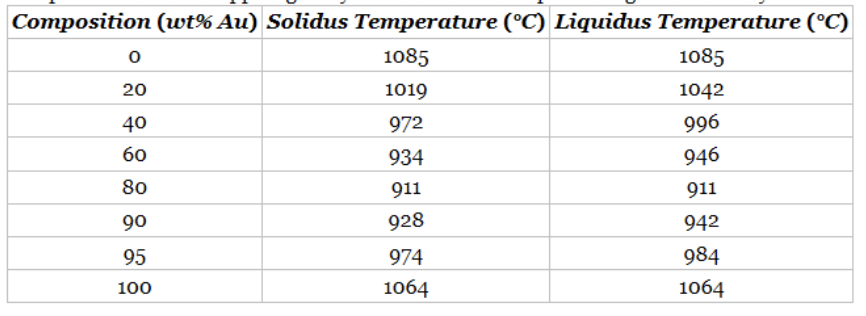
\includegraphics[width=0.5\linewidth]{./figures/f14_1.png}
  \caption{}
  \label{fig:e14_1}
\end{figure}

\exercise{9.5} How many kilograms of nickel must be added to \qty{5,43}{kg} of copper to yield a solidus temperature of \qty{1200}{\celsius}?
